\section{Schobers on a non-characteristic family of discs}\label{section:families}
In this section, we will define schobers and localized schobers on non-characteristic families of discs over a base $B$. We will work complex analytically.

Let $B\subseteq \bbC^{N-1}$ an open subset with respect to the Euclidean topology, we would like to consider perverse schobers on $\bbC\times B$. It is important that $B$ is a subset of $\bbC^{N-1}$ for the following reason. Recall that given a locally constant perverse sheaf on $B$, the natural operation at $b\in B$ which outputs a vector space is not the stalk, but a microstalk, which requires an additional choice of a quadratic form $q_b$ on $T_bB$. Different choices of $q_b$ are related by a Maslov class. For perverse sheaves, we can avoid this choice by taking the ordinary stalk and shifting by $\dim(B)$.

This shifted stalk operation is not available to us in the categorified setting, so we are forced to choose quadratic forms on tangent spaces of $B$. We believe that the work of Nadler--Shende \cite{nadlerSheafQuantizationWeinstein2022}*{\S 10.4} provides a suitable categorification of the Maslov class, organizing how different choices of $q_b$ are related.

We will take the following simpler but less canonical approach. We fix once and for all, compatible choices of quadratic form at each point $b\in B$, which is possible since $\bbC^{N-1}$ admits such a choice. This lets us ignore subtleties involving the Maslov class for the rest of the paper.

\begin{defn}\label{defn:nonchar}
    A non-characteristic family of discs over an open subset $B\subseteq \bbC^{N-1}$ is a pair $(\bbC\times B,H)$ where $H\subset \bbC\times B$ is a hypersurface such that
    \begin{enumerate}
        \item $H\inclto \bbC\times B\xto{\pi} B$ is finite,
        \item there exists a complement of divisors $B^{\opname{sm}}\subseteq B$ such that $H^{\sm}:=H\cap\pi^{-1}(B^{\opname{sm}})\to B^{\opname{sm}}$ is \'etale, and
        \item the closure $\Lambda_H$ of $T^*_{H^{\sm}}$ is non-characteristic for the projection $\pi:\bbC\times B\to B$.
    \end{enumerate}
    Moreover, if we can take $B^{\sm}=B$, then we say that $(\bbC\times B,H)$ is a locally constant family of discs.
\end{defn}

\begin{eg}
    Let $B=\bbC_x$ and denote by $y$ the coordinate of the fibers so that a family of discs is described by some curve $C\subset \bbC^2_{x,y}$. Then, the non-charactericity condition is equivalent to asking that no tangent lines to $C$, or limits thereof, are vertical. For example, $C=\{y^2=x^3\}$ defines a non-characteristic family of discs. A non-example is $\{y^2=x\}$ which has a vertical tangent at $(0,0)$.
\end{eg}

\begin{eg}
    For any $B$, we have the locally constant family of discs, $(\bbC\times B,0\times B)$.
\end{eg}

We informally state the main definitions of this section.

\begin{defn}\label{defn:family1}
    Let $(\bbC\times B,H)$ be a locally constant family of discs. A perverse schober $\calF$ on $(\bbC\times B,H)$ is the data of a locally constant choice of object $\calF\resto{b}$ for each $b\in B$. Denote the collection of such objects by $\sftwoP(\bbC\times B,H)$.
\end{defn}

By applying $\FS_{\sftwoP}$ on each fiber, we obtain a mapping,
\[\FS_{\sftwoP}:\sftwoP(\bbC\times B,H)\to \sftwoP(\bbC\times B,0\times B).\]

\begin{defn}\label{defn:family2}
    Let $(\bbC\times B,H)$ be a non-characteristic family of discs and choose $B^{\opname{sm}}\subseteq B$ as in Definition~\ref{defn:nonchar}. A perverse schober on $(\bbC\times B,H)$ consists of the following data.
    \begin{enumerate}
        \item A perverse schober $\calF\resto{B^{\opname{sm}}}\in \sftwoP(\bbC\times B^{\opname{sm}},H^{\sm})$.
        \item An extension of
        \[\FS_{\sftwoP}(\calF\resto{B^{\opname{sm}}})\in \sftwoP(\bbC\times B^{\opname{sm}},0\times B^{\opname{sm}})\]
        to an object
        \[\FS_{\sftwoP}(\calF)\in \sftwoP(\bbC\times B,0\times B).\]
    \end{enumerate}
\end{defn}

\begin{rmk}\label{rmk:comparison2}
    Definition~\ref{defn:family2} is motivated by, and can be considered a categorification of \cite{gelfandMicrolocalPerverseSheaves2005}*{Proposition 3.3}. This statement is a consequence of an existing definition of perverse sheaves, while for us it is the definition.
\end{rmk}

In \S\ref{subsection:universal} and \S\ref{subsection:schobersonfamily}, we will upgrade $\sftwoP(\bbC\times B,H)$ to a $\two$-category, where $(\bbC\times B,H)$ is a locally constant or non-characteristic family of discs. A key input to our theory is the following consequence of Theorem~\ref{thm:merge}.

\begin{prop}\label{prop:FSisfaithful}
    The functor $\FS_{\sftwoP}:\sftwoP(\bbC,R)\to \sftwoP(\bbC,0)$ is 2-faithful.
\end{prop}

Using this, we will show that Definition~\ref{defn:family2} is independent of the choice of $B^{\sm}$, and in particular agrees with Definition~\ref{defn:family1} for locally constant families. We will also show that whenever $B$ is contractible and $b\in B^{\sm}$, then the restriction functor
\[\sftwoP(\bbC\times B,H)\to \sftwoP(\bbC,H_b)\]
is 2-fully faithful, and identify the image in terms of certain periodicity properties. This is closely related to the periodic SODs as studied in \cite{dyckerhoffNsphericalFunctorsCategorification2023}. We use this to give explicit descriptions of schobers on locally constant families of discs in several examples.

The statements and definitions of \S\ref{subsection:schobersonfamily} admit analogues for both localized and prelocalized schobers.

\begin{rmk}\label{rmk:comparison}
    It is instructive to consider the real analog, where Definition~\ref{defn:family2} fails to define the correct category. Namely, let $L$ be a singular support condition on $\bbR^2_{x,y}$ which is non-characteristic over $y$, and locally constant on $\bbR_x^{\opname{sm}}$. There is a functor,
    \[\sh(\bbR^2_{x,y},L)\to \sh(\bbR_{y}\times \bbR_x^{\opname{sm}},L\resto{\bbR_x^{\opname{sm}}})\times_{\sh(\bbR_{y}\times \bbR_x^{\opname{sm}},0\times \bbR_x^{\opname{sm}})}\sh(\bbR_{y}\times \bbR_x,0\times \bbR_x).\]
    This fails to be an equivalence. For example, compare the following two singular supports. Let $L_1$ be the union of the conormal of the lines $y=x$ and $y=-x$. Let $L_2$ be the union of the conormals to $y=0$ and $y=x^2$. These singular supports define non-equivalent categories, but are indistinguishable on the right hand side of the above expression.

    This comes down to the failure of Proposition~\ref{prop:FSisfaithful} in the real setting. Concretely, the functor which maps a filtered complex of vector spaces to its total space is not faithful.

    Said more conceptually, in the real setting, Morse groups in different Morse indices can admit interesting connecting maps, while in the complex setting, all ``Morse categories'' live in middle index and don't admit such maps between them.
\end{rmk}

In \S\ref{subsection:y2x3}, we study in detail schobers supported on the curve $y^2=x^3$. We show that our definition decategorifies correctly to perverse sheaves as studied by MacPherson--Vilonen \cite{macphersonPerverseSheavesSingularities1988}. We also show that our definition agrees with a microlocalization of $\bbA_2$-schobers as defined by Dyckerhoff--Wedrich \cite{dyckerhoffPerverseSchobersCoxeter2025}, and deduce a relation to $A_2$-configurations of spherical objects of Seidel--Thomas \cite{seidelBraidGroupActions2000}.

\subsection{Schobers on the universal family of discs}\label{subsection:universal}
In this section, we will define a local system of $\two$-categories over the configuration space of $n$ distinct points on $\bbC$, which will be important in what follows.

Let $\Conf(n)$ denote the configuration space parametrizing $n$ distinct points on $\bbC$. Then, the assignment
\[R\in\Conf(n)\mapsto\sftwoP(\bbC,R)\]
upgrades to a local system of $\two$-categories on $\Conf(n)$, which we denote $\ul{\sftwoP}(\bbC,-)$. Moreover, $\FS_{\sftwoP}:\sftwoP(\bbC,R)\to\sftwoP(\bbC,0)$ upgrades to a map of local systems,
\[\ul{\sftwoP}(\bbC,-)\to \ul{\sftwoP}(\bbC,0),\]
where $\ul{\sftwoP}(\bbC,0)$ denotes the constant local system with fibers $\sftwoP(\bbC,0)$.

Fixing $R\in\Conf(n)$, it is well known that $\pi_1(\Conf(n),R)\simeq \Br_R$ is a braid group. So by transport, we obtain a group action $\Br_R\actson \sftwoP(\bbC,R)$.
\begin{prop}\label{prop:intertwines}
    The functor $\FS_{\sftwoP}:\sftwoP(\bbC,R)\to \sftwoP(\bbC,0)$ is naturally $\Br_R$-equivariant, where $\sftwoP(\bbC,0)$ is given the trivial action.
\end{prop}

\begin{cor}\label{cor:discrete}
    The fibers of $\FS_{\sftwoP}:\sftwoP(\bbC,R)\to \sftwoP(\bbC,0)$ are discrete.
\end{cor}

\begin{proof}
    This is immediate from Proposition~\ref{prop:FSisfaithful} together with the fact that $\FS_{\sftwoP}$ is also conservative.
\end{proof}

By combining Proposition~\ref{prop:intertwines} and Corollary~\ref{cor:discrete}, the following definition makes sense.

\begin{defn}\label{defn:periodic2}
    Let $\calG\in\sftwoP(\bbC,R)$. Given $\sigma\in\Br_R$, say that $\calG$ is $\sigma$-periodic if $\calG$ is a fixed point for the $\Br_R$-action acting on the fiber of $\FS_{\sftwoP}$ over $\FS_{\sftwoP}(\calG)$. For a subgroup $H\subseteq \Br_R$, say that $\calG$ is periodic for $H$ if for all $\sigma\in H$, $\calG$ is $\sigma$-periodic.
\end{defn}

We relate the group actions $\Br_R\actson \sftwoP(\bbC,R)$ and $\Br_n\actson \sfSph(n)$, and thus relate Definition~\ref{defn:periodic2} to the notion of periodic SODs given in Definition~\ref{defn:periodic}. We first study the geometry. We claim that $\Cuts(\bbC,R)$ admits in addition to the right torsor action of $\Br_n$, a commuting action of $\Br_R$ by the transport along $\Conf(n)$. A choice $K\in\Cuts(\bbC,R)$ determines
\begin{itemize}
    \item an identification $\sftwoP(\bbC,R)\simeq \sfSph(n)$,
    \item and a group isomorphism $\Br_R\xto{u} \Br_n$ defined by $\sigma\cdot K\simeq K\cdot u(\sigma)$.
\end{itemize}
The actions $\Br_R\actson \sftwoP(\bbC,R)$ and $\Br_n\actson \sfSph(n)$ are identified via these two identifications.

\begin{rmk}
    This is formally similar to the following elementary scenario. Consider a set $S$ of cardinality $n$, and let $\opname{Bij}$ be the set of bijections $f:\{1,\dots,n\}\to S$. Then, $\opname{Bij}$ has a right action by $\Sym_n$ and a left action by $\Sym_S$, by pre- and post-composition respectively. A choice $f\in \opname{Bij}$ determines an isomorphism of groups, $\Sym_S\xto{u} \Sym_n$ defined by the property that for all $\sigma\in\Sym_S$, $\sigma\circ f = f\circ u(\sigma)$.
\end{rmk}

\subsection{The \texorpdfstring{$\two$}{2}-category of schobers on a family of discs}\label{subsection:schobersonfamily}
We upgrade Definition~\ref{defn:family1} and Definition~\ref{defn:family2} to $\two$-categories.

Suppose that $(\bbC\times B,H)$ is a locally constant family of discs, with $B$ connected. Let $f:B\to \Conf(n)$ be the map $b\mapsto H_b$. We define
\[\sftwoP(\bbC\times B,H) := \Gamma(B,f^*\ul{\sftwoP}(\bbC,-)).\]
We can take the enhanced Fukaya--Seidel functor in families, to obtain a functor,
\[\FS_{\sftwoP}:\sftwoP(\bbC\times B,H)\to \sftwoP(\bbC\times B,0\times B).\]

Suppose now that $(\bbC\times B,H)$ is a non-characteristic family of discs. We define the $\two$-category of perverse schobers on $(\bbC\times B,H)$ as the following fibered product of $\two$-categories.
% https://q.uiver.app/#q=WzAsNCxbMCwwLCIyXFxzZlAoXFxiYkNcXHRpbWVzIEIsXFxMYW1iZGEpIl0sWzEsMCwiMlxcc2ZQKFxcYmJDXFx0aW1lcyBCLDBcXHRpbWVzIEIpIl0sWzEsMSwiMlxcc2ZQKFxcYmJDXFx0aW1lcyBCXntcXG9wbmFtZXtzbX19LDBcXHRpbWVzIEJee1xcb3BuYW1le3NtfX0pIl0sWzAsMSwiMlxcc2ZQKFxcYmJDXFx0aW1lcyBCXntcXG9wbmFtZXtzbX19LFIpIl0sWzAsMV0sWzEsMiwiLVxccmVzdG97Ql57XFxvcG5hbWV7c219fX0iXSxbMCwzXSxbMywyLCJcXEZTX3syXFxzZlB9IiwyXV0=
\[\begin{tikzcd}
    {\sftwoP(\bbC\times B,H)}\pullback & {\sftwoP(\bbC\times B,0\times B)} \\
    {\sftwoP(\bbC\times B^{\opname{sm}},H^{\sm})} & {\sftwoP(\bbC\times B^{\opname{sm}},0\times B^{\opname{sm}})}
    \arrow[from=1-1, to=1-2]
    \arrow[from=1-1, to=2-1]
    \arrow["{-\mid_{B^{\opname{sm}}}}", from=1-2, to=2-2]
    \arrow["{\FS_{\sftwoP}}"', from=2-1, to=2-2]
\end{tikzcd}\]

The following statements both use Proposition~\ref{prop:FSisfaithful}.

\begin{prop}\label{prop:restrict}
    Suppose $B$ is contractible and let $(\bbC\times B,H)$ be a non-characteristic family of discs. Fix $b\in B^{\opname{sm}}$. Then, the restriction functor
    \[-\resto{b}:\sftwoP(\bbC\times B,H)\to \sftwoP(\bbC,H_b)\]
    is 2-fully faithful. Moreover, the image is the full sub-$\two$-category
    \[\sftwoP(\bbC,H_b)^{\Image(\sigma)\opname{-periodic}}\]
    consisting of perverse schobers $\calG\in \sftwoP(\bbC,H_b)$ which are periodic for the image of the natural group homomorphism $\sigma:\pi_1(B^{\opname{sm}},b)\to\Br_{H_b}$, as defined in Definition~\ref{defn:periodic2}.
\end{prop}

\begin{proof}
    Consider the following naturally commuting diagram of $\two$-categories where each square is a pullback square.
    % https://q.uiver.app/#q=WzAsOCxbMCwwLCIyXFxzZlAoXFxiYkNcXHRpbWVzIEIsXFxMYW1iZGEpIl0sWzEsMCwiXFxzZlEiXSxbMSwxLCJcXHNmUV57XFxvcG5hbWV7c219fSJdLFswLDEsIjJcXHNmUChcXGJiQ1xcdGltZXMgQl57XFxvcG5hbWV7c219fSxSKSJdLFsyLDAsIjJcXHNmUChcXGJiQ1xcdGltZXMgQiwwXFx0aW1lcyBCKSJdLFsyLDEsIjJcXHNmUChcXGJiQ1xcdGltZXMgQl57XFxvcG5hbWV7c219fSwwXFx0aW1lcyBCXntcXG9wbmFtZXtzbX19KSJdLFsxLDIsIjJcXHNmUChcXGJiQyxSX2IpIl0sWzIsMiwiMlxcc2ZQKFxcYmJDLDApIl0sWzAsMV0sWzEsMiwiXFxvcG5hbWV7S30iXSxbMCwzXSxbMywyLCJcXG9wbmFtZXtJfSIsMl0sWzEsNF0sWzIsNV0sWzQsNSwiLVxcbWlkX3tCXntcXG9wbmFtZXtzbX19fSJdLFs2LDddLFs1LDcsIi1cXG1pZF9iIl0sWzIsNiwiXFxvcG5hbWV7TH0iXSxbNCw3LCJcXG9wbmFtZXtKfSIsMCx7ImN1cnZlIjotNX1dLFszLDYsIi1cXG1pZF9iIiwyLHsiY3VydmUiOjJ9XV0=
    \[\begin{tikzcd}
        {\sftwoP(\bbC\times B,H)}\pullback & \sfQ\pullback & {\sftwoP(\bbC\times B,0\times B)} \\
        {\sftwoP(\bbC\times B^{\opname{sm}},H^{\sm})} & {\sfQ^{\opname{sm}}}\pullback & {\sftwoP(\bbC\times B^{\opname{sm}},0\times B^{\opname{sm}})} \\
        & {\sftwoP(\bbC,H_b)} & {\sftwoP(\bbC,0)}
        \arrow["{\opname{I}'}", from=1-1, to=1-2]
        \arrow[from=1-1, to=2-1]
        \arrow[from=1-2, to=1-3]
        \arrow["{\opname{K}}", from=1-2, to=2-2]
        \arrow["{-\mid_{B^{\opname{sm}}}}", from=1-3, to=2-3]
        \arrow["{\opname{J}}", curve={height=-80pt}, from=1-3, to=3-3]
        \arrow["{\opname{I}}", from=2-1, to=2-2]
        \arrow["{-\mid_b}"', curve={height=12pt}, from=2-1, to=3-2]
        \arrow[from=2-2, to=2-3]
        \arrow["{\opname{L}}", from=2-2, to=3-2]
        \arrow["{-\mid_b}", from=2-3, to=3-3]
        \arrow["{\FS_{\sftwoP}}", from=3-2, to=3-3]
    \end{tikzcd}\]
    Here, $\sfQ$ and $\sfQ^{\opname{sm}}$ are defined by the pullback squares. 
    
    %Make a pointed choice of cuts $(\theta,K)$ for $(\bbC,R_b)$. By Proposition~\ref{prop:infrared}, 
    %An object of $\sfQ^{\opname{sm}}$ is given by a pair $(\calC,\calG)$ consisting of a perverse schober 
    %\[\calC\in \sftwoP(\bbC\times B^{\opname{sm}},0\times B^{\opname{sm}}),\]
    %together with a lift $\calG\in\sftwoP(\bbC,R_b)$ of $\calC\resto{b}$. 
    
    %the data of an SOD $\Upsilon$ of the vanishing cycle of $\calG\resto{b}$, conjugate-compatible with the twist functor $T$ in $\calG\resto{b}$.
    
    From Proposition~\ref{prop:FSisfaithful}, Proposition~\ref{prop:faithful} and Lemma~\ref{lem:faithfulpullback}, we learn that $\opname{I}$ is 2-fully faithful. %Equivalently, the $\two$-category $\mathfrak{L}$ of lifts of $(\calC,\calG)$ to an object $\calF\in \sftwoP(\bbC\times B^{\opname{sm}},R)$ is either the trivial $\two$-category $\pt$ or empty. 
    By pullback square, $\opname{I}':\sftwoP(\bbC\times B,H)\to \sfQ$ is also fully faithful. Since $B$ is contractible, the functor $\opname{J}$ is an equivalence. By base change, the composition $\opname{L}\circ\opname{K}:\sfQ\to \sftwoP(\bbC,H_b)$ is also an equivalence. Composing, we learn that $\opname{L}\circ\opname{K}\circ \opname{I}'$ is fully faithful. Moreover this is identified with
    \[-\resto{b}:\sftwoP(\bbC\times B,H)\to \sftwoP(\bbC,H_b).\]
    
    %Let $\mathfrak{S}$ denote the $\two$-category of all lifts of $\calC\resto{b}$ to an object of $\sftwoP(\bbC,R_b)$. There is a homotopy action of the loop group $\Omega_b B^{\opname{sm}}$ on $\mathfrak{S}$. Our given data provides a point $\calG\in\mathfrak{S}$, and $\mathfrak{L}$ is equivalent to the $\two$-category of fixed-point structures of $\calG$.
    
    %By Corollary~\ref{cor:discrete}, $\mathfrak{S}$ is actually a discrete space. %Indeed, once we make a choice of pointed cut, Proposition~\ref{prop:infrared} implies that $\mathfrak{S}$ is equivalent to the collection of SODs of the vanishing cycle of $\calC\resto{b}$, conjugate-compatible with an autoequivalence.
    %So being a fixed point is a property (and not additional structure) and we deduce that $\mathfrak{L}$ is either contractible or empty as desired. Now the group action factors through the maps
    %\[\Omega_b B^{\opname{sm}}\to ,\]
    
    By Proposition~\ref{prop:faithful}, the essential image of $\opname{I}$ consists of pairs $(\calC,\calG_b)$, where $\calC\in\sftwoP(\bbC\times B^{\opname{sm}},0\times B^{\opname{sm}})$, $\calG\in \sftwoP(\bbC,H_b)$ is a fixed point under the action of $\pi_1(B^{\opname{sm}},b)$ on the space of lifts of $\calC\resto{b}$. The action factors through
    \[\rho:\pi_1(B^{\opname{sm}},b)\to \Br_{H_b},\]
    with $\Br_{H_b}$ acting as described in Definition~\ref{defn:periodic2}. So being a fixed point is equivalent to asking that $\calG_b$ is periodic for the image of $\rho$.
    
    The essential image of functor $\opname{I}'$ consists of objects $\calG\in \sfQ\simeq \sftwoP(\bbC,H_b)$ such that $\opname{K}(\calG)$ lies in the essential image of $\opname{I}$. But
    \[\opname{K}(\calG) = (\calC,\calG),\]
    (where $\calC$ is the trivial local system with fibers $\FS_{\sftwoP}(\calG)$) so we are done.
\end{proof}

\begin{prop}\label{prop:independent}
    Definition~\ref{defn:family2} is independent of the choice of $B^{\sm}$.
\end{prop}

\begin{proof}
    Suppose that $B_1^{\sm}, B_2^{\sm}\subset B$ are two different open subsets which both realize $(\bbC\times B,H)$ as a non-characteristic family of discs. Without loss of generality, we may assume $B_1^{\sm}\subseteq B_2^{\sm}$ and fix a common basepoint $b\in B_1^{\sm}\subseteq B_2^{\sm}$.

    See that the natural map
    \[\pi_1(B_1^{\opname{sm}},b)\to \pi_1(B_2^{\opname{sm}},b)\]
    is surjective. A similar proof to that of Proposition~\ref{prop:restrict} proves the desired result, using Corollary~\ref{cor:surjectivepi1} in the place of Proposition~\ref{prop:faithful}.
\end{proof}

Everything carries over to localized and prelocalized perverse schobers.

\begin{eg}\label{eg:ykxn}
    Let $0<m<n$ be integers. Consider the pair $(\bbC^2_{x,y},C_{m,n})$ where $C_{m,n}$ is the curve $y^m=x^n$. This defines a non-characteristic family of discs over $B=\bbC_x$. We apply Proposition~\ref{prop:restrict} and make a choice of cuts $K$ on the fiber of a fixed basepoint $x_0\in \bbC_x$ to learn that $\sftwoP(\bbC^2_{x,y},C_{m,n})$ is equivalent to the sub-$\two$-category
    \[\sfSph(m)^{n\opname{-periodic}}\subset \sfSph(m),\]
    consisting of objects such that the SOD (on the vanishing cycle of $\FS_{\sfSph}(-)$) is $\tau^n$-periodic where $\tau = \sigma_{m-1}\sigma_{m-2}\cdots \sigma_{1}\in\Br_m$. Here, we recall from the end of \S\ref{subsection:universal} that the choice of cuts $K$ identifies $\Br_{C_{m,n}|_{x_0}}$ with $\Br_m$.
\end{eg}

\begin{eg}\label{eg:waldhausen3}
    We continue Example~\ref{eg:waldhausen1} and Example~\ref{eg:waldhausen2}, carrying over notation. We recall that from a spherical adjunction $F$, we constructed an object of $\sfSph(n)$ via the spherical adjunction $S_{n-1}(F)$.
    
    We then gave a non-abstract interpretation of this and proposed that $S_{n-1}(F)$ comes from a pushforward along $f_0(z)=z^n$, and that lifts to $\sfSph(n)$ come from a factorization
    \[\sftwoP(\bbC_z,0)\xto{(f_x)_*} \sftwoP(\bbC_y,R_x)\xto{\FS_{\sftwoP}} \sftwoP(\bbC_y,0).\]
    We expect that these organize into an object of $\sftwoP(\bbC^2_{x,y},y(y^{n-1}-x^n))$. Applying Proposition~\ref{prop:restrict}, this expectation can concretely be interpreted as a specific periodicity property on the SOD of the vanishing cycle $\calA'$ of $S_{n-1}(F)$. When $n=2$, this is the 4-periodicity of the SOD $\langle\calA,\calB\rangle$ which is well known, see for example \cite{dyckerhoffSphericalAdjunctionsStable2021}*{Proposition 2.5.12}. For general $n$, this is periodicity for $\sigma^n$, where for example if $n=5$, then $\sigma$ is the braid illustrated below.
    \[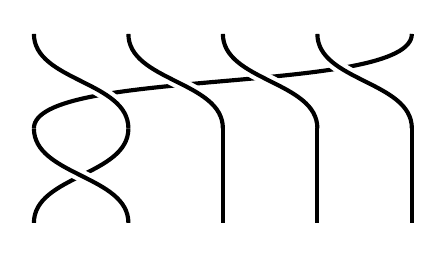
\begin{tikzpicture}[scale=1.2]
        % Strand style definitions
        \tikzset{
            strand/.style={black, line width=1.5pt},
            mask/.style={white, line width=4.5pt}
        }

        % ==========================================
        % TOP BRAID (y = 2 to y = 1)
        % ==========================================
        % Background strand: Strand 5 moves to Position 1 around the back
        \draw[strand] (5, 2) .. controls (5, 1.35) and (1, 1.65) .. (1, 1);

        % Foreground strands (1->2, 2->3, 3->4, 4->5) drawn over strand 5
        \draw[mask] (4, 2) .. controls (4, 1.5) and (5, 1.5) .. (5, 1);
        \draw[strand] (4, 2) .. controls (4, 1.5) and (5, 1.5) .. (5, 1);

        \draw[mask] (3, 2) .. controls (3, 1.5) and (4, 1.5) .. (4, 1);
        \draw[strand] (3, 2) .. controls (3, 1.5) and (4, 1.5) .. (4, 1);

        \draw[mask] (2, 2) .. controls (2, 1.5) and (3, 1.5) .. (3, 1);
        \draw[strand] (2, 2) .. controls (2, 1.5) and (3, 1.5) .. (3, 1);

        \draw[mask] (1, 2) .. controls (1, 1.5) and (2, 1.5) .. (2, 1);
        \draw[strand] (1, 2) .. controls (1, 1.5) and (2, 1.5) .. (2, 1);

        % ==========================================
        % BOTTOM BRAID (y = 1 to y = 0)
        % ==========================================
        % Straight strands at positions 3, 4, 5
        \draw[strand] (3, 1) -- (3, 0);
        \draw[strand] (4, 1) -- (4, 0);
        \draw[strand] (5, 1) -- (5, 0);

        % Position 2 -> Position 1 (under/back)
        \draw[strand] (2, 1) .. controls (2, 0.5) and (1, 0.5) .. (1, 0);

        % Position 1 -> Position 2 (over/front)
        \draw[mask] (1, 1) .. controls (1, 0.5) and (2, 0.5) .. (2, 0);
        \draw[strand] (1, 1) .. controls (1, 0.5) and (2, 0.5) .. (2, 0);

    \end{tikzpicture}\]
    This is more fundamentally described as the braid which rotates the $n$ roots of $y(y^{n-1}-1)=0$ by $\frac{2\pi i}{n-1}$.

    A proof of this expectation can be deduced from \cite{dyckerhoffNsphericalFunctorsCategorification2023}*{Theorem 5.4.2}. One first shows that $\sigma\cdot\frakS=\tau_{n-1}(\frakS)$, where $\tau_{n-1}$ is the autoequivalence coming from the paracyclic structure constructed in \cite{dyckerhoffSphericalAdjunctionsStable2021}. Now, $\tau_{n-1}^n=\Sigma^2$ (\cite{dyckerhoffSphericalAdjunctionsStable2021}*{Discussion following Proposition 3.1.3}) is the double suspension, so that $\sigma^n\cdot\frakS = \frakS$.

    %In \cite{gargGITRootStacks2026}, motivated by work of Bodzenta and Donovan \cite{bodzentaRootStacksPeriodic2024}, a certain 2-term SOD $\frakT$ of $\calA'$ is shown to be $2n$-periodic. This SOD is the one obtained from $\frakS$ by merging all terms except the first. We interpret the periodicity as follows. The braid $\sigma^{n-1}$ exhibits the full-twist braid on the 2-term SOD, and so $n$ times the full-twist is exhibited by $\sigma^{n(n-1)}$, which fixes $\frakS$ and hence $\frakT$. It is instructive to compare this to the proof of \cite{bodzentaRootStacksPeriodic2024}*{Theorem 4.3}.
\end{eg}

\begin{eg}\label{eg:y2x2localized}
    Consider the pair $(\bbC_{x,y}^2,C_{2,2})$ where $C_{2,2}$ is defined in Example~\ref{eg:ykxn}. This is simply the union of two lines, $y=\pm x$. We compute $\olsftwoP(\bbC^2_{x,y},C_{2,2})$. By Proposition~\ref{prop:restrict} (with a fixed pointed choice of cuts), $\olsftwoP(\bbC_{x,y}^2,C_{2,2})$ is equivalent to the sub-$\two$-category of $\sfAut(2)^{\opname{2-periodic}}\subset \sfAut(2)$, given by objects such that the SOD $\Phi=\langle\Phi_1,\Phi_2\rangle$ is $2$-periodic.

    Being $2$-periodic is equivalent to asking that $\Phi_1$ is both left and right orthogonal to $\Phi_2$. In other words, $\Phi=\Phi_1\oplus\Phi_2$. The autoequivalence $T$ also splits $T=T_1\oplus T_2$, where $T_i$ is an autoequivalence of $\Phi_i$.

    Thus there is an equivalence,
    \[\sfAut(2)^{\opname{2-periodic}}\simeq \sfAut \oplus \sfAut.\]
    We note that in the setting of \cite{dyckerhoffNsphericalFunctorsCategorification2023}, an SOD being 2-periodic is equivalent to the gluing functor being zero, which yields the same conclusion.

    Geometrically, we interpret this as the observation that the Legendrian $\Lambda_{C_{2,2}}^\infty$ is a disjoint union of two smooth Legendrians.
\end{eg}

\begin{eg}\label{eg:y2x3localized}
    Consider the pair $(\bbC_{x,y}^2,C_{2,3})$ where $C_{2,3}$ is defined in Example~\ref{eg:ykxn}. We compute $\olsftwoP(\bbC^2_{x,y},C_{2,3})$. We apply Proposition~\ref{prop:restrict} to learn that $\olsftwoP(\bbC_{x,y}^2,C_{2,3})$ is equivalent to the sub-$\two$-category of $\sfAut(2)^{\opname{3-periodic}}\subset \sfAut(2)$, given by objects such that the SOD $\Phi=\langle\Phi_1,\Phi_2\rangle$ is $3$-periodic.

    By Example~\ref{eg:aut2}, an object in the image is given by the data of a 3-periodic functor $F:\Phi_1\to\Phi_2$ admitting all adjoints, autoequivalences $T_1,T_2$ of $\Phi_1$, $\Phi_2$ respectively, together with an equivalence, $F\circ T_1\simeq T_2\circ F^{RR}$.

    It is shown in \cite{dyckerhoffNsphericalFunctorsCategorification2023} that a functor $F$ is 3-periodic if and only if it is an equivalence. In particular, $F^{RR}\simeq F$, and so $T_1$ and $T_2$ are identified via $F$. So the data is equivalent to just giving a single pair $(\Phi_1,T_1)$, defining an equivalence,
    \[\sfAut(2)^{\opname{3-periodic}}\simeq \sfAut.\]

    Geometrically, we interpret this as the observation that $\Lambda_{C_{2,3}}^\infty$ is a smooth Legendrian. We will further interpret this as an instance of Radon transform in Example~\ref{eg:yx3}.
\end{eg}

\begin{rmk}\label{rmk:cerf}
    There is a fruitful analogy between perverse schobers on $(\bbC_y,R)$ and Picard-Lefschetz theory, with sheaves on $(\bbR,L)$ and Morse theory, where $L$ is a singular support condition containing the zero section and containing only covectors in non-negative codirections.

    We extend this analogy to schobers on a family of discs, $(\bbC^2_{x,y},C)$, non-characteristic over $B=\bbC_x$. This is analogous to Cerf theory, which concerns how generic families of Morse functions may degenerate. In the classical theory, there are two types of Cerf singularities, called exchange singularities and birth-death singularities.

    The families of (localized) perverse schobers appearing in Example~\ref{eg:y2x2localized} and Example~\ref{eg:y2x3localized} can be thought of as analogues of these two types of singularities.
\end{rmk}

\subsection{Schobers supported on a cuspidal cubic}\label{subsection:y2x3}
We make a detailed study of the category $\sftwoP(\bbC^2_{x,y},C_{2,3})$, where the $C_{2,3}$ is the curve $y^2=x^3$.

The category of perverse sheaves microsupported along the associated Lagrangian $\Lambda_{C_{2,3}}$ is described by MacPherson--Vilonen \cite{macphersonPerverseSheavesSingularities1988}*{Proposition 3.1}, which we recall below. We aim to show that our definition categorifies this.

\begin{prop}\label{prop:mv}
    Let $A=\bbC\langle a_1,a_2\rangle/(a_1a_2a_1 -a_1^2 +a_1, a_2a_1a_2 -a_2^2 +a_2)$. Then, the category $\Perv(\bbC^2_{x,y},C_{2,3})$ is equivalent to the abelian category of $A$-modules such that $1-a_1$ and $1-a_2$ are invertible.
\end{prop}

We show that our definition of $\sftwoP(\bbC^2_{x,y},C_{2,3})$ decategorifies to Proposition~\ref{prop:mv}. Note however that we must be in the setting of large categories in order to use Proposition~\ref{prop:KLisEM}, although it is not clear if this is necessary.

\begin{prop}\label{prop:y2x3description}
    The $\two$-category $\sfSph(2)^{\opname{3-periodic}}$ is equivalent to the $\two$-category whose objects are $(\Psi,F_1,F_2)$, where
    \begin{itemize}
        \item $\Psi$ is a stable category and
        \item $F_1,F_2$ are spherical monads on $\Psi$ with units $u_i:\id\to F_i$,
    \end{itemize}
    such that the following squares are Cartesian.
    \[\begin{tikzcd}
        {F_1F_1} & {F_1F_2F_1} \\
        {F_1} & 0
        \arrow["{1\circ u_2\circ 1}"', from=1-1, to=1-2]
        \arrow["{m_1}", from=1-1, to=2-1]
        \arrow[from=1-2, to=2-2]
        \arrow[from=2-1, to=2-2]
    \end{tikzcd}
    \begin{tikzcd}
        {F_2F_2} & {F_2F_1F_2} \\
        {F_2} & 0
        \arrow["{1\circ u_1\circ 1}"', from=1-1, to=1-2]
        \arrow["{m_2}", from=1-1, to=2-1]
        \arrow[from=1-2, to=2-2]
        \arrow[from=2-1, to=2-2]
    \end{tikzcd}
    \]
    In particular, taking $K$-theory yields a perverse sheaf microsupported on $C_{2,3}$ via Proposition~\ref{prop:mv}.
\end{prop}

We begin with a straightforward description of $\sftwoP(\bbC^2_{x,y},C_{2,3})$.

\begin{lem}\label{lem:y2x3easy}
    The $\two$-category $\sftwoP(\bbC^2_{x,y},C_{2,3})$ is equivalent to the $\two$-category whose objects are $(\Phi_1,\Phi_2,\Psi,S_1,S_2)$, consisting of
    \begin{itemize}
        \item stable categories $\Phi_1,\Phi_2,\Psi$, and
        \item spherical functors $S_i:\Phi_i\to \Psi$ for $i=1,2$,
    \end{itemize}
    such that $S_1^RS_2$ is an equivalence.
\end{lem}

\begin{proof}
    By Example~\ref{eg:ykxn}, we have an equivalence,
    \[\sftwoP(\bbC^2_{x,y},C_{2,3})\simeq \sfSph(2)^{\opname{3-periodic}}.\]
    We recall from \cite{dyckerhoffNsphericalFunctorsCategorification2023} that a 2-term SOD is 3-periodic if and only if its gluing functor is an equivalence. The (Cartesian) gluing functor here is $S_1^RS_2$.
\end{proof}

\begin{proof}[Proof of Proposition~\ref{prop:y2x3description}]
    We begin with the description of Lemma~\ref{lem:y2x3easy}. We deduce from $S_1^RS_2$ being invertible that $S_1$ is conservative so we can describe $\Phi_1$ monadically in terms of $\Psi$, as discussed in \S\ref{subsection:prelocalized} (although the role of $\Phi,\Psi$ are reversed). We have likewise for $\Phi_2$. Thus, an object of $\sftwoP(\bbC^2_{x,y},C_{2,3})$ is equivalent to the data of
    \begin{itemize}
        \item a stable category $\Psi$,
        \item spherical monads $F_1,F_2$ on $\Psi$,
        \item such that $S_1^RS_2$ is an equivalence,
    \end{itemize}
    where $S_i:\Mod_{\Psi}(F_{i})\to\Psi$ is the forgetful functor, so that $F_{i} = S_iS_i^L$.

    We use the notation
    \[S_i^LS_i\to 1\to T_i\xto{+1}\]
    for relevant twist functors, so that $T_iS_i^R[-1]\isomto S_i^L$.

    To ask for $S_1^RS_2$ to be an equivalence is equivalent to asking that
    \begin{enumerate}
        \item\label{item:unit} the unit $1\to S_1^RS_2S_2^LS_1$ is an equivalence, and
        \item\label{item:counit} the counit $S_2^LS_1S_1^RS_2\to 1$ is an equivalence.
    \end{enumerate}
    We begin with (\ref{item:unit}). We post-compose with $T_i[-1]$ and ask instead that
    \[T_1[-1]\to S_1^LS_2S_2^LS_1\]
    is an equivalence.

    We use a strategy similar to the proof of Proposition~\ref{prop:sphmonad} in order to rewrite the last condition in terms of the monads. By Proposition~\ref{prop:KLisEM}, $S_i^L$ is (stably) essentially surjective. Also, $S_1$ is conservative, so we may post-compose and pre-compose by these respectively. So we ask that
    \[S_1T_1S_1^L[-1]\to S_1S_1^LS_2S_2^LS_1S_1^L\]
    is an equivalence. Rewriting this in terms of monads, condition (\ref{item:unit}) is equivalent to asking that the first of the squares in the statement is Cartesian. Similarly, condition (\ref{item:counit}) is equivalent to asking that the second square is Cartesian.
\end{proof}

We next relate our description to the framed $\bbA_2$-schobers defined by Dyckerhoff--Wedrich \cite{dyckerhoffPerverseSchobersCoxeter2025}. We recall the definition here.

\begin{defn}\label{defn:dw}
    A framed $\bbA_2$-schober is given by a commuting square of stable categories,
    \[\begin{tikzcd}
        {\calA_{3}} & {\calA_{1,2}} \\
        {\calA_{2,1}} & {\calA_{1,1,1}}
        \arrow["I", from=1-1, to=1-2]
        \arrow["H"', from=1-1, to=2-1]
        \arrow["F"', from=1-2, to=2-2]
        \arrow["G", from=2-1, to=2-2]
    \end{tikzcd}\]
    such that
    \begin{enumerate}
        \item all functors admit right adjoints,
        \item $F,G$ are spherical,
        \item the cones of the Beck--Chevalley maps $HI^R \to G^RF, IH^R\to F^RG$ are equivalences,
        \item certain Beck--Chevalley squares (\cite{dyckerhoffPerverseSchobersCoxeter2025}*{(2.3.3),(2.3.4)}) are Cartesian, and
        \item the cotwist $T_3:\calA_3\to\calA_3$ (\cite{dyckerhoffPerverseSchobersCoxeter2025}*{Example 3.26}) is an equivalence.
    \end{enumerate}
    We denote by $\sftwoP^{\opname{DW}}(\bbA_2)$ the $\two$-category of $\bbA_2$-schobers.
\end{defn}

\begin{prop}\label{prop:agreeswithdw}
    The $\two$-category $\sftwoP(\bbC^2_{x,y},C_{2,3})$ is equivalent to the full sub-$\two$-category of $\sftwoP^{\opname{DW}}(\bbA_2)$ consisting of $\bbA_2$-schobers such that $\calA_{3}=0$.
\end{prop}

\begin{proof}
    An $\bbA_2$-schober with $\calA_{3}=0$ is given by a diagram of stable categories,
    \[\begin{tikzcd}
        {} & {\calA_{1,2}} \\
        {\calA_{2,1}} & {\calA_{1,1,1}}
        \arrow["F"', from=1-2, to=2-2]
        \arrow["G", from=2-1, to=2-2]
    \end{tikzcd}\]
    such that
    \begin{enumerate}
        \item all functors admit all repeated adjoints,
        \item $F,G$ are spherical,
        \item the compositions $G^RF$ and $F^RG$ are equivalences,
        \item certain Beck--Chevalley squares (\cite{dyckerhoffPerverseSchobersCoxeter2025}*{(2.3.3),(2.3.4)}) are Cartesian, and
        \item the cotwist $T_3:\calA_3\to\calA_3$ is an equivalence.
    \end{enumerate}
    One checks that the condition on Beck--Chevalley squares follows from the remaining ones. The cotwist invertibility is trivially satisfied. So we recover the description given in Lemma~\ref{lem:y2x3easy}.
\end{proof}

We can interpret Proposition~\ref{prop:agreeswithdw} as follows. We think of $\bbA_2$-schobers as a candidate for perverse schobers on $(\bbC^2_{x,y},C_{2,3}\cup T^*_{0}\bbC^2)$. Their singular support condition differs from $\Lambda_{C_{2,3}}$ by the conormal at zero. The ``microstalk'' at a point here is $\calA_{3}$, so we may ``microlocalize'' to $\Lambda_{C_{2,3}}$ by setting this to zero, providing a candidate for perverse schobers on $(\bbC^2,C_{2,3})$. Proposition~\ref{prop:agreeswithdw} verifies that this candidate agrees with our definition. In fact, this sub-$\two$-category is enough to encode the $A_2$-configurations as discussed in \cite{dyckerhoffPerverseSchobersCoxeter2025}*{\S 3.6}. 

\begin{eg}\label{eg:y2x3geometry}
    Let $k=\bbC$. Consider for each $x\neq0$, the perverse schober coming from a symplectic fibration,
    \[\calF_x := \calF(\bbC_u,\frac12(u^3-3xu))\in\sftwoP(\bbC_y,R_x).\]
    Here, $R_x=\Crit(\frac12(u^3-3xu))=\{\pm x^{3/2}\}$. This defines an object
    \[\calF\resto{\bbC_x-0}\in\sftwoP((\bbC_x-0)\times\bbC_y,y^2=x^3).\]
    In order to extend over $x=0$, we must exhibit a trivialization of $\FS_{\sftwoP}(\calF_x)$.

    The category underlying $\FS_{\sftwoP}(\calF_x)$ is exactly the Fukaya--Seidel category (in the original sense) of the pair $(\bbC_u,\frac12(u^3-3xu))$, where we have chosen a stop in a fixed direction $\theta$. This is independent of $x$ since the leading term $u^3$ is independent of $x$. By varying $\theta$, this exhibits the desired trivialization.

    We can also study this perverse schober by restriction to the fiber $x=1$ via Proposition~\ref{prop:restrict}. After making a pointed choice of cuts from the critical values to a far away point $y_\infty$, we obtain the object of $\sfSph(2)$ given by
    \[S_1,S_2:\Vect\to \Fuk(u^3-3u=y_\infty),\]
    where $S_1,S_2$ are two vanishing cycles. These vanishing cycles famously intersect once, so that $S_2^RS_1:\Vect\to \Vect$ is an equivalence. By Lemma~\ref{lem:y2x3easy}, this defines a perverse schober on $(\bbC^2,C_{2,3})$.
\end{eg}

We expect that a similar story continues to hold for $\bbA_N$-schobers, by observing that the discriminant locus $\Delta\subset \bbC^{N-1}\sslash \Sym_N$ defines a non-characteristic family of discs by treating the $N$\ts{th} elementary symmetric polynomial as the fiber coordinate. More generally, we expect that from a perverse schober on $(\bbC^{N+1},H)$, we may produce a (perverse) local system of categories on $\bbC^{N+1}-H$, so that we obtain an action of $\pi_1(\bbC^{N+1}-H,p_0)$ on the nearby cycles category at $p_0\in\bbC^{N+1}-H$.